\scanpage{12}
Donnée de $q$ équivaut \unsure{:|à} \unsure{l|la} donnée de $\sigma\in\operatorname{Aut}^{\pm1}(\unsure{G|Z},T)$
\[
\left\{\begin{aligned}p(\sigma)&=-1\\ \sigma^2&=1\end{aligned}\right.
\]
\[
\begin{aligned}
&q_t(-1)=\sigma_t\\[.5em]
&\sigma_{tg}=g\,\sigma_t\,g^{-1}
=g\,\underbrace{\sigma_t\,g^{-1}\,\sigma_t^{-1}}_{g}\,\sigma_t
=g^2\,\sigma_t=\sigma_t\,g^{-2}\\[-.3em]
&\hspace{.53\linewidth}\boxed{\sigma_{tg}=g^2\sigma_t=\sigma_t g^{-2}}
\end{aligned}
\]

\uline{Corollaire} Si $n$ impair, $t\longmapsto\deleted{\unsure{q}}\sigma_t$ est une bijection de $T$ avec l'ens \deleted{\unsure{des}} $p^{-1}\{-1\}$; donc si on a un \unsure{pol.|pl.} à un nb impair de cotés, l'applic\textsuperscript{n} $t\longmapsto\sigma_t$ qui, à tt sommet du polygone, associe l'unique autom non orienté qui fixe ce sommet, est bijection.

\uline{NB} Si $n$ pair, \deleted{\unsure{elle}} ce n'est pas bijectif, \deleted{mais} \deleted{\unsure{pour tt}} ses fibres sont vides ou de cardinal 2\ldots

% slanted left margin note; lettering rises approximately 30 degrees to the right.
% Coordinates below preserve the distinct upper rule and the sweeping lower enclosure.
\reversemarginpar
\margin{\hspace*{-2cm}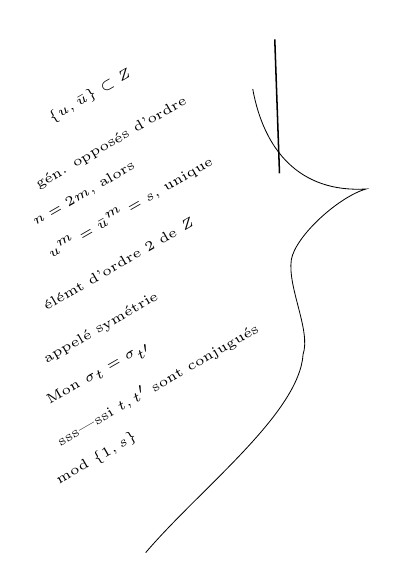
\begin{tikzpicture}[x=.01cm,y=.01cm,every node/.style={inner sep=0pt,outer sep=0pt,anchor=base west,font=\tiny,rotate=30}]
\path[use as bounding box] (0,0) rectangle (440,675);
\node at (30,555) {$\{u,\bar u\}\subset Z$};
\node at (14,470) {\unsure{gén.} opposés d'ordre};
\node at (10,423) {$n=2m$, alors};
\node at (30,382) {$u^m=\bar u^m=s$, \uline{unique}};
\node at (24,315) {\uline{\unsure{élémt} d'ordre} 2 de $Z$};
\node at (24,248) {appelé symétrie};
\node at (28,196) {Mon $\sigma_t=\sigma_{t'}$};
\node at (42,143) {\unsure{sss|ssi} $t,t'$ sont \unsure{conjugués}};
\node at (40,95) {mod $\{1,s\}$};
\draw[line width=.55pt] (314,660) -- (320,490);
\draw[line width=.3pt] (286,597)
 .. controls (300,520) and (345,465) .. (430,470)
 .. controls (395,460) and (340,410) .. (335,380)
 .. controls (330,345) and (360,290) .. (350,260)
 .. controls (345,185) and (220,90) .. (150,8);
\end{tikzpicture}}

\uline{Sommet} \uline{opposé}, symétrie canonique

\uline{Parenthèse}\qquad Produit fibré d'ens

\diagram{\begin{tikzpicture}
\node[anchor=north west,inner sep=0pt] (square) at (0,0) {\begin{tikzcd}[ampersand replacement=\&,column sep=2em,row sep=2.4em]
E\arrow[r,"p"] \& \unsure{S|B}\\
P\arrow[u,dashed,"q'"]\arrow[r,dashed,"p'"] \& F\arrow[u,"q"']
\end{tikzcd}};
% The set description begins at the level of the lower row of the square.
\node[anchor=north west,inner sep=0pt] at (4.5,-1.5) {$\begin{aligned}
&P\subset E\times F\\[-.4em]
&\hspace{.3em}\rotatebox{90}{$=$}\\[-.4em]
&\{(x,y)\mid px=qy\}
\end{aligned}$};
\end{tikzpicture}}

% Detached, definite ink stroke above Solution; no lexical value is assigned.
\figure{\makebox[\linewidth][l]{
\begin{tikzpicture}[x=1cm,y=1cm]
\fill (0.025,0.29) .. controls (-0.015,0.28) and (-0.012,0.19) .. (0.018,0.15)
 .. controls (0.038,0.12) and (0.039,0.075) .. (0.012,0.055)
 .. controls (-0.005,0.039) and (-0.036,0.055) .. (-0.043,0.037)
 .. controls (-0.044,0.008) and (0.003,-0.004) .. (0.028,0.022)
 .. controls (0.071,0.06) and (0.06,0.12) .. (0.05,0.17)
 .. controls (0.072,0.23) and (0.062,0.27) .. (0.025,0.29) -- cycle;
\end{tikzpicture}}}

Solution d'un Pb universel dans la cat. des ens :

Si $E,F,S$ des \unsure{grpes|groupes}, $p,q$ hom de grpe, alors $P$ un \unsure{grpe|groupe} (et solution du pb univ. analogue ds cat. des \unsure{grpes|groupes})
\[
\operatorname{Ker}p\sim\operatorname{Ker}p',\quad
\operatorname{Ker}q\sim\operatorname{Ker}q'
\]

Si \tikz[baseline=(p.base)]{\node[inner sep=0pt] (p) at (0,0) {$p$};
\node[anchor=base west,inner sep=0pt] (sur) at (.45,0) {surjectif};
\node[anchor=base west,inner sep=0pt] at (.40,.5) {\inserted{$:E\mathbin{\text{---}}S$}};
\draw[line width=.35pt] (.42,.13) .. controls (.62,.35) and (1.0,.34) .. (1.5,.48);
} bijectif) alors $P\mathbin{\text{---}}F$ surjectif bijectif).

[Langage des \tikz[baseline=(old.base)]{\node[inner sep=0pt] (old) {\deleted{\unsure{diagrammes}}};
\node[anchor=south,inner sep=0pt] at ([yshift=.5ex]old.north) {\inserted{carrés}};
} cartésiens]

Image inverse d'ex. de \unsure{grpe|groupe|grpes|groupes}
% archive sheet number: 11
